
\chapter*{The 2-D Wave Equation With Staggered Leapfrog}
\addcontentsline{toc}{chapter}{The 2-D Wave Equation With Staggered Leapfrog} 
\section*{Two dimensional grids}
\addcontentsline{toc}{section}{Two dimensional grids} 

	\marginpar{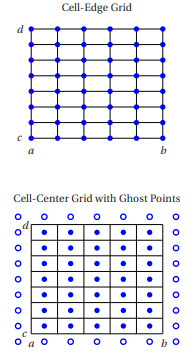
\includegraphics[width=\marginparwidth]{fig61}\captionof{figure}{Two types of 2-D grids.}\label{fig:29}}
In this lab we will do problems in two spatial dimensions, $x$ and $y$, so we need
to spend a little time thinking about how to represent 2-D grids. For a simple
rectangular grid where all of the cells are the same size, 2-D grids are pretty
straightforward. We just divide the $x$-dimension into equally sized regions and
the $y$-dimension into equally sized regions, and the two one dimensional grids
intersect to create rectangular cells. Then we put grid points either at the corners
of the cells (cell-edge) or at the centers of the cells (cell-centered). On a cell-center
grid we\rq ll usually want ghost point outside the region of interest so we can get the
boundary conditions right. \\ NumPy has a nice way of creating rectangular two-dimensional grids using
the meshgrid command. You can create 2-d rectangle defined by $x \in [a,b]$ and
$y \in [c,d]$ and then plot a function on that grid this way:
\begin{lstlisting}
from mpl_toolkits.mplot3d import Axes3D
import matplotlib.pyplot as plt
from matplotlib import cm
import numpy as np
# Make 1D x and y arrays
Nx=20
a=-1.5
b=1.5
x,hx = np.linspace(a,b,Nx,retstep = True)
Ny=10
c=-1.2
d=1.2
y,hy = np.linspace(c,d,Ny,retstep = True)
# Make the 2D grid and evaluate a function
X, Y = np.meshgrid(x,y,indexing='ij')
Z = X**2 + Y**2
# Plot the function as a surface.
fig = plt.figure(1)
ax = fig.gca(projection='3d')
surf = ax.plot_surface(X, Y, Z, cmap=cm.viridis)
plt.xlabel('x')
plt.ylabel('y')
fig.colorbar(surf)
\end{lstlisting}
The argument $indexing='ij'$ in the meshgrid function switches the ordering
of the elements in the resulting matrices from the matrix indexing convention
$Z[row,col]$ to the function indexing convention $Z[x_i,y_y]$ for representing $Z(x_i, y_i)$.

\paragraph*{P6.1} 

\begin{enumerate}[label=(\alph*)]
\item
Use the code fragment above in a program to create a 30-point celledge grid in $x$ and a 50-point cell-edge grid in $y$ with $a = 0, b = 2,
c = −1, d = 3$. Switch back and forth between $indexing='ij'$ and
$indexing='xy'$, and look at the different matrices that result. Convince the TA that you know what the difference is. (HINT: When
we write matrices, rows vary in the $y$ dimension and columns vary
in the $x$ direction, whereas with $Z(x_i, y_i)$ we have a different convention. NumPy\rq s naming convention seems backward to us, but
we didn\rq t come up with it. Sorry.) We recommend that you use the
$indexing='ij'$ convention, as it tends to more readable code for representing $Z(x_i, y_i)$.
\item  Using this 2 - D grid, evaluate the following function of $x$ and $y$:
\begin{equation}\label{eq:61}
f(x,y) = e^{-(x^2+y^2)} \cos(5\sqrt{x^2+y^2})
\end{equation}
Use the $plot_surface$ command to make a surface plot of this function. Properly label the $x$ and $y$ axes with the symbols $x$ and $y$, to get
a plot like Fig. 6.2.
\end{enumerate}
There are a lot more options for plotting surfaces in Python, but we\rq ll let you
explore those on your own. For now, let\rq s do some physics on a two-dimensional
grid.
\section*{The two-dimensional wave equation}
\addcontentsline{toc}{section}{The two-dimensional wave equation}


	\marginpar{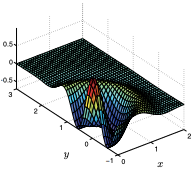
\includegraphics[width=\marginparwidth]{fig62}\captionof{figure}{Plot from Problem $6.1$. The graphic in this figure was created with Matlab. Python\rq s graphics engine is sort of privative in comparison to Matlab\rq s, so you won\rq t get something quite so nice. In particular, getting the scaling right is painful in Python.}\label{fig:30}}
The wave equation for transverse waves on a rubber sheet is
\begin{equation}\label{eq:62}
\mu \frac{\partial^2 z}{\partial t^2} = \sigma (\frac{\partial^2 z}{\partial x^2} + \frac{\partial^2 z}{\partial y^2} )
\end{equation}
In this equation $\mu$ is the surface mass density of the sheet, with units of mass/area.
The quantity $\sigma$ is the surface tension, which has rather odd units. By inspecting
the equation above you can find that σ has units of force/length, which doesn\rq t
seem right for a surface. But it is, in fact, correct as you can see by performing the
following thought experiment. Cut a slit of length $L$ in the rubber sheet and think
about how much force you have to exert to pull the lips of this slit together. Now
imagine doubling $L$; doesn\rq t it seem that you should have to pull twice as hard to close the slit? Well, if it doesn\rq t, it should; the formula for this closing force is
given by $\sigma L$, which defines the meaning of $\sigma$.
We can solve the two-dimensional wave equation using the same staggered
leapfrog techniques that we used for the one-dimensional case, except now we
need to use a two dimensional grid to represent $z(x, y,t)$. We\rq ll use the notation $ z^n_{j,k} = z(x_j,y_k,t_n) $ to represent the function values. With this notation, the
derivatives can be approximated as
\begin{equation}\label{eq:63}
\frac{\partial^2 z}{\partial t^2} \approx \frac{z^{n+1}_{j,k}-2z^n_{j,k}+z^{n-1}_{j,k}}{\tau^2} )
\end{equation}
\begin{equation}\label{eq:64}
\frac{\partial^2 z}{\partial x^2} \approx \frac{z^{n}_{j+1,k}-2z^n_{j,k}+z^{n}_{j-1,k}}{h^2_x} )
\end{equation}\\
\begin{equation}\label{eq:65}
\frac{\partial^2 z}{\partial y^2} \approx \frac{z^{n}_{j,k+1}-2z^n_{j,k}+z^{n}_{j,k-1}}{h^2_y} )
\end{equation}
where $h_x$ and $h_y$ are the grid spacings in the $x$ and $y$ dimensions. We insert these
three equations into Eq. \eqref{eq:62} to get an expression that we can solve for z at the
next time (i.e. $z^{n+1}_{j,k} $). Then we use this expression along with the discrete version
of the initial velocity condition
\begin{equation}\label{eq:66}
v_0(x_j,y_k)\approx \frac{z^{n+1}_{j,k}-z^{n-1}_{j,k}}{2\tau}
\end{equation}
to find an expression for the initial value of $z^{n-1}_{j,k}$ (i.e. $zold$) so we can get things
started.
\paragraph*{P6.2} 

\begin{enumerate}[label=(\alph*)]
	\item Derive the staggered leapfrog algorithm for the case of square cells
with $h_x = h_y = h$. Write a program that animates the solution of the
two dimensional wave equation on a square region that is $[−5,5] ×
[−5,5]$ and that has fixed edges. Use a cell-edge square grid with
the edge-values pinned to zero to enforce the boundary condition.
Choose $\sigma = 2 N/m$ and $ \mu = 0.3 kg/m^2$
and use a displacement initial
condition that is a Gaussian pulse with zero velocity

\begin{equation}\label{eq:67}
z(x,y,0) = e^{-5(x^2+y^2)}
\end{equation}

This initial condition doesn\rq t strictly satisfy the boundary conditions,
so you should pin the edges to zero.
Getting the animation to work can be tricky, so here is a framework of
code for the animation loop:
\begin{lstlisting}
from mpl_toolkits.mplot3d import Axes3D
import matplotlib.pyplot as plt
import numpy as np
# your code to initialize things
tfinal=10
t=np.arange(0,tfinal,tau)
skip=10
fig = plt.figure(1)
# here is the loop that steps the solution along
for m in range(len(t)):
# Your code to step the solution
# make plots every skip time steps
if m % skip == 0:
plt.clf()
ax = fig.gca(projection='3d')
surf = ax.plot_surface(X,Y,z)
ax.set_zlim(-0.5, 0.5)
plt.xlabel('x')
plt.ylabel('y')
plt.draw()
plt.pause(0.1)
\end{lstlisting}
	\marginpar{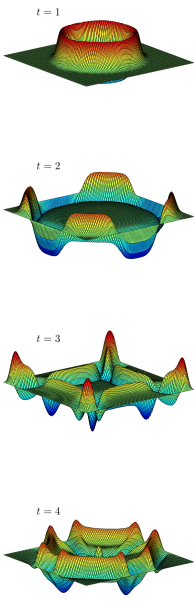
\includegraphics[width=\marginparwidth]{fig63}\captionof{figure}{A wave on a rubber sheet with fixed edges.}\label{fig:31}}
Run the simulation long enough that you see the effect of repeated
reflections from the edges.
\item You will find that this two-dimensional problem has a Courant condition similar to the one-dimensional case, but with a factor out front:
\begin{equation}\label{eq:68}
\tau < fh \sqrt{\frac{\mu}{\sigma}}
\end{equation}
where $\sqrt{\frac{\mu}{\sigma}}$ is the wave speed and $f$ is an arbitrary constant. Determine the value of the constant $f$ by numerical experimentation.
(Try various values of $\tau$ and discover where the boundary is between
numerical stability and instability.)
\item Also watch what happens at the center of the sheet by making a plot
of $z(0,0,t)$ there. In one dimension the pulse propagates away from
its initial position making that point quickly come to rest with $z = 0$.
This also happens for the three-dimensional wave equation. But
something completely different happens for an even number of dimensions; you should be able to see it in your plot by looking at the
behavior of $z(0,0,t)$ before the first reflection comes back.
\item Finally, change the initial conditions so that the sheet is initially flat
but with the initial velocity given by the Gaussian pulse of Eq. \eqref{eq:67}.
In one dimension when you pulse the system like this the string at
the point of application of the pulse moves up and stays up until
the reflection comes back from the ends of the system. (We did this
experiment with the slinky in Lab 5.) Does the same thing happen
in the middle of the sheet when you apply this initial velocity pulse?
Answer this question by looking at your plot of $z(0,0,t)$. You should
find that the two-dimensional wave equation behaves very differently
from the one-dimensional wave equation.


\end{enumerate}
\section*{Elliptic, hyperbolic, and parabolic PDEs}
\addcontentsline{toc}{section}{Elliptic, hyperbolic, and parabolic PDEs}

Let\rq s step back and look at some general concepts related to solving partial differential equations. Three of the most famous PDEs of classical physics are

\begin{enumerate}[label=(\roman*)]
\item Poisson\rq s equation for the electrostatic potential $V (x, y)$ given the charge
density $ρ(x, y)$
\begin{equation}\label{eq:69}
\frac{\partial^{2} V}{\partial x^{2}}+\frac{\partial^{2} V}{\partial y^{2}}=\frac{-\rho}{\epsilon_{0}}+\text { Boundary Conditions }
\end{equation}
\item The wave equation for the wave displacement $y(x,t)$
\begin{equation}\label{eq:610}
\frac{\partial^{2} y}{\partial x^{2}}-\frac{1}{c^{2}} \frac{\partial^{2} y}{\partial t^{2}}=0+\text { Boundary Conditions }
\end{equation}
\item The thermal diffusion equation for the temperature distribution $T(x,t)$ in a
medium with diffusion coefficient $D$
\begin{equation}\label{eq:611}
\frac{\partial T}{\partial t}=D \frac{\partial^{2} T}{\partial x^{2}}+\text { Boundary Conditions }
\end{equation}
\end{enumerate}
To this point in the course, we\rq ve focused mostly on the wave equation, but over
the next several labs we\rq ll start to tackle some of the other PDEs. \\
Mathematicians have special names for these three types of partial differential
equations, and people who study numerical methods often use these names, so
let\rq s discuss them a bit. The three names are elliptic, hyperbolic, and parabolic.
You can remember which name goes with which of the equations above by remembering the classical formulas for these conic sections:
\begin{equation}\label{eq:612}
\text{ellipse:} \frac{x^{2}}{a^{2}}+\frac{y^{2}}{b^{2}}=1
\end{equation}
\begin{equation}\label{eq:613}
\text{hyperbola:} \frac{x^{2}}{a^{2}}-\frac{y^{2}}{b^{2}}=1
\end{equation}
\begin{equation}\label{eq:614}
\text{parabola:} y=a x^{2}
\end{equation}
Compare these equations with the classical PDE\rq s above and make sure you can use their resemblances to each other to remember the following rules: Poisson\rq s equation is elliptic, the wave equation is hyperbolic, and the diffusion equation is parabolic. These names are important because each different type of equation requires a different type of algorithm and boundary conditions. \\  Elliptic equations require the same kind of boundary conditions as Poisson\rq s equation: $V (x, y)$ specified on all of the surfaces surrounding the region of interest. Notice that there is no time delay in electrostatics. When all of the bounding voltages are specified, Poisson\rq s equation says that $V(x, y)$ is determined instantly throughout the region surrounded by these bounding surfaces. Because of the finite speed of light this is incorrect, but Poisson\rq s equation is a good approximation to use in problems where things happen slowly compared to the time it takes light to cross the computing region. \\
To understand hyperbolic boundary conditions, think about a guitar string
described by the transverse displacement function $y(x,t)$. It makes sense to
give spatial boundary conditions at the two ends of the string, but it makes no
sense to specify conditions at both $t = 0$ and $t = t_{final}$ because we don\rq t know the
displacement in the future. This means that you can\rq t pretend that $(x,t)$ are like
$(x, y)$ in Poisson\rq s equation and use \lq\lq surrounding\rq\rq -type boundary conditions. But
we can see the right thing to do by thinking about what a guitar string does. With
the end positions specified, the motion of the string is determined by giving it an
initial displacement $y(x,0)$ and an initial velocity $\partial y(x,t)/ \partial t\vert_{t=0}$, and then letting
the motion run until we reach the final time. So for hyperbolic equations the
proper boundary conditions are to specify end conditions on y as a function of
time and to specify the initial conditions $y(x,0)$ and $\partial y(x,t)/ \partial t\vert_{t=0}$. \\

Parabolic boundary conditions are similar to hyperbolic ones, but with one difference. Think about a thermally-conducting bar with its ends held at fixed
temperatures. Once again, surrounding-type boundary conditions are inappropriate because we don\rq t want to specify the future. So as in the hyperbolic case,
we can specify conditions at the ends of the bar, but we also want to give initial conditions at $t = 0$. For thermal diffusion we specify the initial temperature
$T (x,0)$, but that\rq s all we need; the \rq\rq velocity\lq\lq $\partial T / \partial t$ is determined by Eq. \eqref{eq:611},
so it makes no sense to give it as a separate boundary condition. Summarizing:
for parabolic equations we specify end conditions and a single initial condition
$T (x,0)$ rather than the two required by hyperbolic equations. \\ 

If this seems like an arcane side trip into theory, we\rq re sorry, but it\rq s important.
When you numerically solve partial differential equations you will spend 10 \%
of your time coding the equation itself and 90 \% of your time trying to make the
boundary conditions work. It\rq s important to understand what the appropriate
boundary conditions are. \\
Finally, there are many more partial differential equations in physics than
just these three. Nevertheless, if you clearly understand these basic cases you
can usually tell what boundary conditions to use when you encounter a new one.
Here, for instance, is Schr{\"o}dinger\rq s equation:
\begin{equation}\label{eq:615}
i \bar{h} \frac{\partial \psi}{\partial t}=-\frac{\bar{h}^{2}}{2 m} \frac{\partial^{2} \psi}{\partial x^{2}} + V \psi
\end{equation}
which is the basic equation of quantum (or \rq\rq wave\lq\lq) mechanics. The wavy nature
of the physics described by this equation might lead you to think that the proper
boundary conditions on $\psi (x,t)$ would be hyperbolic: end conditions on $\psi$ and initial conditions on $\psi$ and $\partial \psi / \partial t$. But if you look at the form of the equation, it
looks like thermal diffusion. Looks are not misleading here; to solve this equation
you only need to specify $\psi$ at the ends in x and the initial distribution $ \psi(x,0)$, but
not its time derivative. And what are you supposed to do when your system is both hyperbolic and
parabolic, like the wave equation with damping?
\begin{equation}\label{eq:616}
\frac{\partial^{2} y}{\partial x^{2}}-\frac{1}{c^{2}} \frac{\partial^{2} y}{\partial t^{2}}-\frac{1}{D} \frac{\partial y}{\partial t}=0
\end{equation}
The rule is that the highest-order time derivative wins, so this equation needs
hyperbolic boundary conditions
\paragraph*{P6.3} Make sure you understand this material well enough that you are comfortable answering basic questions about PDE types and what types of
boundary conditions go with them on a quiz and/or an exam. Then explain
it to the TA to pass this problem off.
